\documentclass{ctexart}
\usepackage{multicol}
\usepackage{amsmath, amsfonts, amssymb}
\usepackage{tikz, tkz-graph}
\usepackage{subfigure}
\usepackage{geometry}
\special{dvipdfmx:config z 0} % delete this when release

\usetikzlibrary{positioning}

\geometry{a4paper,scale=0.8}

\title{集合论与图论~作业10-11}
\author{庄嘉毅}
\date{October 2022}

\def\QED{\hfill $\square$}
\def\st{\textrm{s.t.}\,}
\def\pair#1{\left\langle #1 \right\rangle}
\def\conj{\mathrel{\wedge}}
\def\disj{\mathrel{\vee}}
\def\equ{\mathrel{\Leftrightarrow}}
\def\restr{\mathbin{\upharpoonright}}
\def\ple{\mathrel{\preccurlyeq}}
\DeclareMathOperator{\dom}{dom}
\DeclareMathOperator{\ran}{ran}
\DeclareMathOperator{\fld}{fld}
\DeclareMathOperator{\card}{card}
\DeclareMathOperator{\e}{e}

\everymath{\displaystyle}
% \linespread{2}

\begin{document}

\maketitle

\section*{习题七}

\paragraph*{1} 设 $G$ 有 $n$ 个顶点, 由握手定理,
$2\times 16\le 3\times 4+4\times 3 + 2(n-3-4)=2n+10$,
解得 $n\ge 11$.

\begin{figure}[ht]
    \centering
    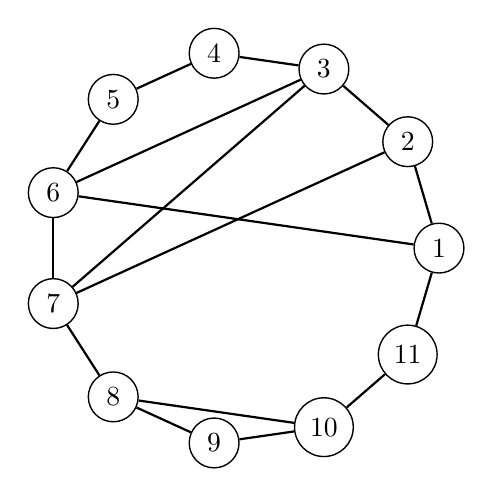
\begin{tikzpicture}
        \GraphInit[vstyle=Normal]
        \Vertices[unit=2.5]{circle}{1,2,3,4,5,6,7,8,9,10,11}
        \Edges(1,2,3,4,5,6,7,8,9,10,11,1)
        \Edges(1,6,3)
        \Edges(2,7)
        \Edges(3,7)
        \Edges(10,8)
    \end{tikzpicture}
    \caption{第1题图}
    \label{fig:1}
\end{figure}

如图 \ref{fig:1} 所示,存在 11 个顶点的图满足条件,因此顶点数的最小值为11.

\paragraph*{2} 设 $G$ 有 $n$ 个5度顶点, $9-n$个6度顶点, 由握手定理,
$5n+6(9-n)\equiv 0\pmod 2$, 故 $2\mid n$, 因此 $n\ne 5$,
即 $n\ge 6$ 或 $n\le 4$ , 也即 $n\ge 6$ 或 $9-n\ge 5$. \QED


\paragraph*{3} 记多面体有 $f$个面,每个面的棱数分别为$e_1,e_2,\ldots,e_f$,
由握手定理,
\begin{gather*}
    \sum_{i=1}^f e_i \equiv 0 \pmod 2
\end{gather*}

若 $e_i$ 均为奇数, 那么
\begin{gather*}
    \sum_{i=1}^f e_i \equiv \sum_{i=1}^f 1 \equiv f \pmod 2
\end{gather*}

故此时 $f$ 只能为偶数. 因此不存在有奇数个面且每个面均有奇数条棱的多面体. \QED

\paragraph*{5} 由握手定理, $3n=2m$, 又 $2n-3=m$, 解得 $n=6,m=9$.

\begin{figure}[ht]
    \centering
    \subfigure[]{
        \label{fig:5a}
        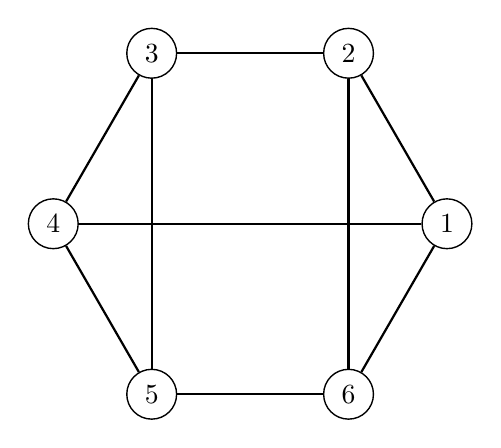
\begin{tikzpicture}
            \GraphInit[vstyle=Normal]
            \Vertices[unit=2.5]{circle}{1,2,3,4,5,6}
            \Edges(1,2,3,4,5,6,1,4)
            \Edges(2,6)
            \Edges(3,5)
        \end{tikzpicture}}
    \quad
    \subfigure[]{
        \label{fig:5b}
        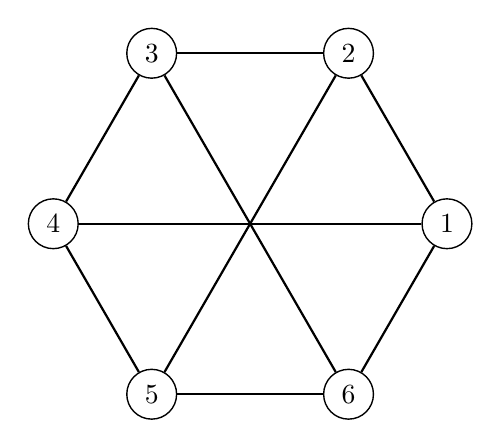
\begin{tikzpicture}
            \GraphInit[vstyle=Normal]
            \Vertices[unit=2.5]{circle}{1,2,3,4,5,6}
            \Edges(1,2,3,4,5,6,1,4)
            \Edges(2,5)
            \Edges(3,6)
        \end{tikzpicture}}
    \caption{第5题图}
    \label{fig:5}
\end{figure}

如图 \ref{fig:5} 所示, 可以构造出两种不同构的图.
以下证明只存在这两种不同构的图.

考虑按图中三角形的数量分类. 若图中不含三角形, 则只有一种(图 \ref{fig:5b}).

若图中存在三角形, 不妨设 $v_1,v_2,v_3$ 为三角形的三个顶点,
那么将此三角形的三边从图中删去后, $v_1,v_2,v_3$的度数变为1,
$v_4,v_5,v_6$的度数仍为3. 此时, $v_4,v_5,v_6$ 的总度数为9,
其中, $v_1,v_2,v_3$至多贡献3, 因此顶点为$v_4,v_5,v_6$的子图里,
至少有$(9-3)/2=3$条边, 即$v_4,v_5,v_6$也构成三角形.
因此, 包含三角形的图只有一种(图 \ref{fig:5a}).

\paragraph*{11} 由于 $G$ 与 $\overline{G}$ 边数相同, 
所以有 $|E(G\cup \overline{G})| =|E(K_n)| =n(n-1)/2 \equiv 0 \pmod 2$, 因此 $n\equiv 0, 1 \pmod 4$.

\paragraph*{14} 使用反证法. 假设结论不成立, 即对于任意 $u,v,w\in V(G)$,
若 $(u,v),(v,w)\in E(G)$, 有 $(u,w)\in E(G)$.

对任意的 $u,v\in V(G)$, 由 $G$ 的连通性, 存在从 $u$ 到 $v$ 的路径,
记路径上的顶点为 $u=u_0,u_1,\ldots,u_k=v$. 

那么, 由假设, 因为 $(u_0,u_1),(u_1,u_2)\in E(G)$, 所以 $(u_0,u_2)\in E(G)$.
进而又因为 $(u_2,u_3)\in E(G)$, 所以 $(u_0,u_3)\in E(G)$.
以此类推, 可以得到 $(u_0,u_k)\in E(G)$, 即 $u$ 到 $v$ 之间存在边.

由 $u$ 和 $v$ 的任意性, 可以得到 $G$ 中任意两点之间存在边,
即 $G$ 是完全图, 与假设矛盾, 因此假设不成立, 结论成立. \QED

\paragraph*{16} 记各圈长度的最大公约数为 $d$. 由 $\delta(G)\ge 3$, 
知存在 $(u,v)\in E(G)$, 对边 $(u,v)$ 进行``扩大路径法'', 
得``极大路径'' $\Gamma=v_0v_1\cdots v_l$.
由 $d(v_0)\ge 3$, 存在 $(v_0,v_i),(v_0,v_j)\in E(G)$, 
其中$1\le i,j\le l$且$i<j$.

此时, $\Gamma_1=v_0v_1\cdots v_iv_0$,
$\Gamma_2=v_0v_1\cdots v_jv_0$,
$\Gamma_3=v_0v_iv_{i+1}\cdots v_jv_0$ 均为 $G$ 中的圈,
其长度均为 $d$ 的倍数, 即 $d\mid i, d\mid j, d\mid(j-i+2)$, 
因此 $d\mid 2$, 即 $d=1$ 或 $d=2$. \QED


\paragraph*{18} 由定理 7.13, $\kappa(G) \ge 2\delta(G)-n+2=k+1$,
故 $G$ 为 $k$-连通图. 取 $k=1$ 的特例, 即 $G$ 为连通图. \QED

\paragraph*{22} 不妨设 $G$ 是块(否则可以只对于$G$的成块子图进行考虑).

若 $|V(G)| =2$, 那么只能有 $G=K_2$. 

若 $|V(G)|\ge 3$, 那么由 $G$ 是块知, $\delta(G)\ge 2$, 
因此 $G$ 中必存在长度至少为 3 的圈 $\Gamma=v_0v_1v_2\cdots v_{l-1}v_0$, 
由条件知此圈为奇圈, 即 $l$ 为奇数. 以下证明: $G=\Gamma$.

首先证明 $V(G)=V(\Gamma)$. 若存在$\Gamma$外的顶点, 
由 $G$ 的连通性, 存在顶点 $u_0\in V(G)-V(\Gamma)$, $v\in V(\Gamma)$, 
使得 $(u_0,v)\in E(G)$. 不妨令 $v=v_0$. 
那么由连通性, $u_0$ 与 $v_1,v_2,\ldots,v_{l-1}$ 间均存在路径,
且至少有一条路径不经过 $v_0$ (否则 $v_0$ 为 $G$ 的割点), 
记这条路径为 $P=u_0u_1\cdots u_kv_i$.
另外记从 $v_0$ 到 $v_i$ 的两条路径分别为
$R_1=v_0v_1v_2\cdots v_i$ 和 $R_2=v_0v_{l-1}v_{l-2}\cdots v_i$.

于是, 在 $G$ 中存在圈 $\Gamma_1=P\cup R_1\cup \{(u_0,v_0)\}$, 
$\Gamma_2=P\cup R_2\cup \{(u_0,v_0)\}$,
其长度分别为 $|\Gamma_1| = k+i+2$, $|\Gamma_2| = k+l-i+2$.
注意到 $|\Gamma_1|+|\Gamma_2| = 2k+l+4\equiv l \pmod 2$,
又 $l$ 为奇数, 故 $|\Gamma_1|$与$|\Gamma_2|$奇偶性不同,
其中必有一个是偶圈, 矛盾. 因此不存在$\Gamma$外的顶点, 
即 $V(G)=V(\Gamma)$.

接下来证明 $E(G)=E(\Gamma)$. 若存在 $\Gamma$ 外的边 $(v_i,v_j)$,
不妨设 $j>i+1$, 可找到 $G$ 的两个圈 
$\Gamma_3=v_0v_1v_2\cdots v_iv_jv_{j+1}\cdots v_{l-1}v_0$ 和
$\Gamma_4=v_iv_{i+1}v_{i+2}\cdots v_jv_i$,
其长度分别为 $|\Gamma_3| = l-j+i+1$ 和 $|\Gamma_4| = j-i+1$,
同上, 有$|\Gamma_3|+|\Gamma_4| = 2l+2\equiv l \pmod 2$,
因此 $|\Gamma_3|$与$|\Gamma_4|$奇偶性不同,
其中必有一个是偶圈, 矛盾. 因此不存在 $\Gamma$ 外的边,
即 $E(G)=E(\Gamma)$.

综上, $G=\Gamma$, 即 $G$ 为 $K_2$ 或奇圈. \QED

\paragraph*{25} 使用反证法. 假设结论不成立, 即 $n$ 阶竞赛图 $D$ 
是传递且强连通的.

取 $\pair{u,v}\in E(D)$, 由 $D$ 的强连通性, 存在从 $v$ 到 $u$ 的通路,
记路径上的顶点为 $v=v_0,v_1,\ldots,v_k=u$. 

那么, 由传递性, 因为 $\pair{v_0,v_1},\pair{v_1,v_2}\in E(D)$, 
所以 $\pair{v_0,v_2}\in E(D)$.
进而又因为 $\pair{v_2,v_3}\in E(D)$, 所以 $\pair{v_0,v_3}\in E(D)$.
以此类推, 可以得到 $\pair{v_0,v_k}\in E(D)$.
而同时已知 $\pair{u,v}\in E(D)$, 与 $D$ 是竞赛图矛盾.
因此假设不成立, 故 $D$ 不是强连通图. \QED

% 教材习题7: 22,25
\end{document}
